%

\section{Energy Consumption of HMOG Features}
\label{sec:power}

%
We measured the energy consumption of two basic modules involved in extracting HMOG features:  (1) sensors (i.e., accelerometer and gyroscope); and (2) feature computation (i.e., calculation of a HMOG feature from raw sensor readings). Our main finding from energy consumption analysis is that decreasing sensor sampling rate (from 100Hz to  as low as 16Hz) considerably reduced the energy overhead without impacting the authentication performance of HMOG features. %


\subsection{Experiment Setup and Design}
\label{sec:powerms}

We developed an Android application that collects and processes sensor data at 
different sampling rates. Our application allows us to selectively enable sensors and HMOG features. We extracted the best-performing 17 features for sitting (i.e., top-ranked 17 features in Figure~\ref{fig:fisherFeaturesSit} that were selected by 10-CV) and 13 HMOG features for walking (i.e., top-ranked 13 features in Figure~\ref{fig:fisherFeaturesWalk}, selected by 10-CV). The union of these two feature sets resulted in 18 HMOG features. Because none of these feature were extracted from magnetometer, we did not measure its energy consumption. 
%
%
%
 
%

%
 

 Experiments were performed using a Samsung Galaxy S4 smartphone running Android 4.4. To obtain consistent and repeatable results, we terminated all other applications 
and all Google services on the smartphone. Additionally, we switched off WiFi, 
Bluetooth, and cellular radios. The screen was turned on during the experiments. 
Automatic brightness adjustments were disabled, and brightness was set to the 
lowest level. We used the Monsoon Power Monitor ~\cite{monsoonPowerMonitor} to 
measure the phone's energy consumption.

We performed the energy consumption experiments as follows. First, we measured baseline energy 
consumption by running our application with all sensors and features disabled. 
Then, we enabled accelerometer and gyroscope, and evaluated the corresponding energy consumption.
Our application is designed to sample sensors at all supported frequencies. In the case of Galaxy S4, the available sampling rates are: 5Hz, 16Hz, 50Hz, and 100Hz. 
We used authentication scan lengths of 60 and 120 seconds. Our results report the average and standard deviation of ten experiments in each setting. 
Finally, we quantified the energy overhead of computing 18 HMOG features from sensor readings acquired during data collection.

\paragraph{Calculation of EERs at Lower Sampling Rates} We originally collected our data at 100Hz sampling rate. In order to obtain the EERs for lower sampling rates, we used downsampling. For example, to simulate 16Hz sampling rate, we choose every sixth sensor reading from the original sensor data. Then, using the downsampled data, we performed HMOG-based authentication with SM verifier for 60- and 120-second scans using the same evaluation process as in Section  \ref{sectionExperiments}. 

\subsection{Energy Consumption of HMOG Authentication}
\label{sec:pr}

%

\paragraph{EERs vs.~Energy Consumption} 
Figure~\ref{fig:eer_diff_rate} shows that  EERs for 16Hz 
sampling rate are comparable to those of 50Hz and 100Hz for both sitting and walking, while the EERs for 5Hz are 
considerably worse than 16Hz, 50Hz, and 100Hz. 

On the other hand, Table \ref{tbl:power_result} shows that energy overhead over the baseline is low (between 
6.2\% and 7.9\%) for 5Hz and
16Hz sampling rates and, in comparison, high (between 12.8\% and 20.5\%) for 50Hz 
and 100Hz. 
%
%
%

%
%
Thus, during the active authentication with HMOG, we can choose 16Hz instead of 
100Hz as the sensor sampling rate, which would lower the energy overhead of 
sensor data collection by about 60\% without sacrificing EER. 

%
%
\paragraph{Energy Consumption for Feature Computation} 
%
The energy overhead for computing 18 
features is very low compared to energy overhead of sensor data collection. The  
energy consumption for computing all 18 HMOG features is 0.08 joules, 
which corresponds to  0.19\% overhead for the 60-second and  0.1\% for  
120-second scans. This low overhead can be attributed to the fact that HMOG features are time-domain 
features. (As suggested by previous 
research~\cite{Krause:2005:TOP:1104998.1105279,Yan:2012:ECA:2357489.2358011}, 
computing time-domain features consumes less energy than computing frequency-domain features.)
Further, because HMOG feature computation involves simple arithmetic calculations, 
they can be processed very quickly by the smartphone's CPU (on average 37ms per feature,  in our case). %


%
%
%
%
%
%
%
%
%
%
%
%

\begin{table}[t]

\centering 
\caption{Energy consumption measurement results.}
\label{tbl:power_result}
\resizebox{1\columnwidth}{!}{
\begin{tabular}{c|llllll|}
{} & \multicolumn{6}{c}{60 Seconds Scan Length} \\
{} & {} & Baseline & 5Hz & 16Hz & 50Hz & 100Hz \\\hline
Energy & Mean & 42.7 & 45.5 & 46.1 & 48.4 & 51.5 \\
Consumption (J) & StdDev & 0.04 & 0.13 & 0.15 & 0.25 & 0.29 \\\hline
{Overhead to Baseline} & {} & N/A & 6.6\% & 7.9\% & 13.3\% & 20.5\% \\
\multicolumn{7}{c}{ }  \\ 
{} &  \multicolumn{6}{c|}{120 Seconds Scan Length} \\ 
{} & {} & Baseline & 5Hz & 16Hz & 50Hz & 100Hz \\\hline
Energy & Mean & 85.6 & 90.9 & 92.1 & 96.5 & 102.9 \\
Consumption (J) & StdDev & 0.17 & 0.21 & 0.23 & 0.30 & 0.36\\\hline
{Overhead to Baseline} & {} & N/A & 6.2\% & 7.6\% & 12.8\% & 20.1\%
\end{tabular}}
\end{table}

%
%
%
%
%
%
%
%
%
%
%
%

\begin{figure}[!htb]
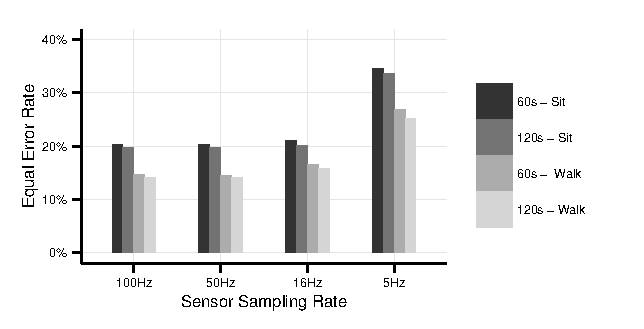
\includegraphics[width=1.1\linewidth]{plots_R/power_sit_walk_bar.pdf}
\caption[]{Performance of HMOG features with different sensor sampling rates using SM verifier.}
\label{fig:eer_diff_rate}
\end{figure}